\chapter{Implementierung}

\section{Die Spieleverwaltung}
\sectionauthor{\frank}

Ziel eines derartigen Frameworks ist, dieses möglichst modular \unsure{Ist das
das Ziel?} zu entwickeln. Dazu gehört auch, es zu ermöglichen, Spiele einfach
und dynamisch hinzufügen zu können. Sicher könnte man dessen benötigten Klassen
erstellen und anschließend an irgendeiner Stelle in die App hardcoden. Doch wir
wollten all das, was zu diesem Prozess gehört, vereinfachen, und damit flüssiger,
angenehmer und vor allem modularer gestalten. Dadurch wird auch das
nachträgliche Ändern oder Löschen von Spielen trivial. Außerdem wird so der Weg
für zukünftige Automatisierung -- wie beispielsweise Spielständen -- geebnet.

\subsection{Deklaration von Spielen}

Die Deklaration und Deklaration von Spiele-Metadaten erfolgt strukturiert in
einer XML-Datei, \emph{games.xml}, welche durch eine \textbf{Document Type
Definition} (\textbf{DTD}) semantisch abgesichert ist. So wird gewährleistet,
dass die Spiele im passenden Format vorliegen, und so entsprechend
weiterverarbeitet werden können. Die Datei erlaubt außerdem die Zuordnung in
selbst gewählte Spiele-Kategorien, wie zum Beispiel \emph{Kartenspiele} oder
\emph{Brettspiele}.

Hier ist ein Auszug der Datei, welcher die verwendete DTD zeigt:

\begin{lstlisting}
<!DOCTYPE games [
    <!ELEMENT games (category*)>
    <!ELEMENT category (game*)>
    <!ATTLIST category id ID #REQUIRED>
    <!ATTLIST category title CDATA #REQUIRED>
    <!ATTLIST category icon CDATA #REQUIRED>
    <!ELEMENT game EMPTY>
    <!ATTLIST game title CDATA #REQUIRED>
    <!ATTLIST game description CDATA #REQUIRED>
    <!ATTLIST game icon CDATA #REQUIRED>
    <!ATTLIST game rules CDATA #REQUIRED>
    <!ATTLIST game tag CDATA #IMPLIED>
    <!ATTLIST game activity CDATA #REQUIRED>
]>
\end{lstlisting}

\subsubsection{Kategorien}
\label{sssec:categories}

Wie man daraus ablesen kann, können unter dem Root-Element \code{games} beliebig
viele Kategorien hinzugefügt werden. Eine solche Kategorie wird beschrieben
durch drei verpflichtende Attribute. \code{id} ist eindeutig im gesamten
Deklarationsbereich, also der Datei zu wählen. Sie wird später weiter verwendet,
um eine Kategorie eindeutig identifizieren und wiederfinden zu können.
\code{title} ist die Bezeichnung dieser Kategorie. Hier ist es möglich, Text aus
der \emph{strings.xml}-Datei zu referenzieren. Solche Referenzierungen werden in
der Form \code{"@strings/ref"} angegeben, wobei \code{ref} für den
entsprechenden Identifikator steht. Außerdem ist noch ein Icon anzugeben, das
später beispielsweise im Navigation Drawer zu finden ist. Hier ist ebenfalls die
Referenzierung einer Resource möglich.

\subsubsection{Spiele}
\label{sssec:games}

Spiele werden analog unterhalb der Kategorien angegeben. Sie besitzen jedoch
unterschiedliche Attribute. \code{title} und \code{icon} stimmen mit der
Funktionalität deren einer Kategorie überein. Ihre Werte kann man
beispielsweise in der Spieleliste \improvement{Das in die Grundlagen} oder in
der Android-Actionbar sehen. Zusätzlich sind die beschreibenden Attribute
\code{description}, \code{rules} hinzuzufügen. Sie werden ebenfalls in
GUI-Elementen der App zu Finden sein. \code{activity} bestimmt später in der
laufenden Anwendung, welche Aktivität gestartet wird, wenn man auf das Spiel in
der Liste klickt. Die Aktivität muss im Package \emph{view} unter
\emph{activity} im Root-Package liegen, um gestartet werden zu können. Sie wird
mit ihrem Ort innerhalb dieses Paketes angegeben, zum Beispiel \emph{``Chess''}
Weitere Unter-Pakete sind möglich. Das letzte Attribut \code{tag} ist zur
genaueren Bestimmung der Eigenschaften eines Spiels gedacht und kann später in
der Aktivität des Spiel selbst abgefragt werden. Mit diesem Tag ist es denkbar,
weitere Varianten eines Spieles anzulegen, ohne dafür neue Aktivitäten
/ Klassen anfertigen zu müssen. Es besteht darüberhinaus die Möglichkeit,
mehrere Tags festzulegen; diese werden durch Verkettungszeichen | getrennt. Im
Falle eines 2-Spieler Schach-960's, lautet der Tag \code{``aiGame|chess960''}.

\subsubsection{Beispiel}

Die Datei mit genauer einer Kategorie und einem Spiel würde also so aussehen:

\begin{lstlisting}
<?xml version="1.0" encoding="utf-8"?>
<games>

    <category
        id="boardgames"
        title="@string/boardgames"
        icon="@drawable/icon_checkerboard">

        <game
            title="@string/game_chess_title"
            description="@string/game_chess_player_vs_ai"
            icon="@mipmap/ic_launcher"
            rules="@string/game_chess_rules"
            tag="aiGame"
            activity="Chess" />

    </category>

</games>
\end{lstlisting}

Die \textbf{DTD} wurde aus Platzgründen weggelassen.

\subsection{Die Spiele-Klasse}

Passend zu der Beschreibung eines Spiels in der XML-Datei gibt es die Klasse
\code{Game}. In ihr befinden sich die äquivalenten Attribute zu denen der
Markup-Datei. Außerdem besitzt diese Klasse eine Instanzmethode \code{boolean
isTaggedWith(String tag)}, welche abfragt, ob das übergebene Argument Teil des
Tags ist. So kann eine Spieleaktivität ganz ohne Umschweife die Eigenschaften
des zugehörigen Elements aus der Deklarationsdatei abfragen, um bestimmte
Abfolgen des Spielverlaufes zu verändern. Siehe \autoref{sssec:games}.

\subsection{Der Spielemanager}

Doch wie kommen die Spieleinformationen in eine \code{Game}-Klasse? Die Antwort
darauf ist die Spieleverwaltung \code{Games}. Dieses Quasi-\textbf{Singleton}
legt beim erstmaligen Initialisieren eine Liste aller Spiele und Kategorien an.
Das geschieht mithilfe des \code{XmlResourceParser}s. Eine Übersicht über die
Klassen- und Dateistruktur findet sich in \autoref{fig:gm_uml}. 

\begin{figure}[h]
	\centering
	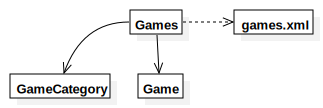
\includegraphics{resources/gamemanager/gamemanager_uml}
	\caption{Gamemanager Übersicht}
	\label{fig:gm_uml}
\end{figure}

\subsubsection{Der XmlResourceParser}

Hierbei handelt es sich um einen einfachen Parser, der es erlaubt, XML-Dokumente
von Anfang bis Ende zu durchlaufen.\\ Zuerst wird die Spiele-Deklarationsdatei
mittels \emph{try-with-resources} aus den Resourcen geladen:

\begin{lstlisting} 
try (XmlResourceParser xmlParser = mContext.getResources().getXml(R.xml.games)) {
	&[\dots]&
} catch (XmlPullParserException | IOException e) {
	&[\dots]&
}
\end{lstlisting}

Anschließend kann der Parser wie ein Iterator durchlaufen werden:

\begin{lstlisting}
int eventType = xmlParser.getEventType();
for (; eventType != XmlPullParser.END_DOCUMENT; eventType = xmlParser.next()) {
    if (eventType != XmlPullParser.START_TAG) continue; &\label{line:starttag}&
\end{lstlisting}

Hierbei interessieren nur die Positionen am Anfang von einem Tag, da man dort
die Attribute eines Tags abfragen kann (Zeile~\ref{line:starttag}). Weitere
Informationen werden nicht benötigt. Jetzt ist es also so, dass der Parser in
der Schleife immer am Anfang eines Tags steht; das ist in unserem Fall entweder
\code{games}, \code{category} oder \code{game}, wobei nur die beiden letzteren
relevant sind. Da diese sich auf der zweiten und dritten Verschachtelungsebene
befinden, ist die Erkennung, um welchen es sich handelt, mit der Abfrage

\begin{lstlisting} 
switch (xmlParser.getDepth()) {
    case 2:
        // Tiefe 2: Kategorie
    case 3:
        // Tiefe 3: Spiel
}
\end{lstlisting}

realisierbar. Nun weiß man also, ob es sich beim aktuellen Element um eine
Kategorie oder ein Spiel handelt. Aufgrund der Tatsache, dass ein Spiel sich
immer unter einer Kategorie befinden muss, kann man sich sicher sein, dass Fall
\code{3} nie eintritt, bevor Fall \code{2} nicht eingetreten ist. Dies erlaubt
uns, in Tiefe 2 Werte zu setzen, welche in Tiefe zwei für ein Spiel gebraucht
werden, ohne zum Beispiel eine \code{NullPointerException} zu werfen. Das können
wir für die Feststellung der Kategorie eines Spiels ausnutzen, denn der
\code{XmlResourceParser} kennt von sich aus keine Beziehungen zwischen den
einzelnen Tags. Die aktuelle Kategorie wird in der Status-Variablen
\code{stateGameCategory} gesichert und anschließend benutzt, wenn ein Spiel in
der Speicherstruktur zusammen mit der Kategorie abgespeichert wird.\\ Bei dem
Versuch ein Objekt der \code{GameCategory} -- oder später der \code{Game} --
Klasse zu erzeugen stößt man nun auf ein Problem: Wie schafft man es, dass aus
dieser Attribut-Liste eine Parameter-Liste für das zu erzeugende Objekt wird?
Und vor allem: Wie kann man diese Liste den \emph{passenden} Argumenten
zuordnen? Da das mit Java nur sehr schwer beziehungsweise unter gewissen
Umständen unmöglich ist, haben wir uns dafür entschieden, die geforderten
Parameter der \code{GameCategory}- und \code{Game}-Klasse redundant im Singleton
als Liste abzulegen. In diesen Listen befinden sich die Attributsnamen aus
\code{games.xml} in der Reihenfolge wie sie der Konstruktor erwartet.\\ Der
Vorgang, eine Kategorie ein Objekt der Klasse \code{GameCategory} umzuwandeln,
sieht also folgendermaßen aus:

\begin{lstlisting}
private final String[] CATEGORY_ATTRIBUTES = {"icon", "id", "title"};
private final List<GameCategory> categories = new ArrayList<>();
private final Map<String, List<Game>> games = new HashMap<>();

&[\dots]&

String[] categoryAttributes = getAttributes(xmlParser, CATEGORY_ATTRIBUTES);
int categoryIcon = AndroidResources.getResourceIDFromString(categoryAttributes[0]);
GameCategory category = new GameCategory(categoryIcon, categoryAttributes[1], categoryAttributes[2]);
stateGameCategory = category.getCategoryId();
categories.add(category);
games.put(stateGameCategory, new ArrayList<Game>());
\end{lstlisting}

Eine Besonderheit befindet sich in diesem Ausschnitt: Die Parameter des
Konstruktors der Klasse haben unterschiedliche Datentypen. Das Icon wird nämlich
nicht als String, sondern als Integer, der eine Drawable-Resource referenziert,
abgespeichert. Da dieses Attribut das erste in \code{CATEGORY\_ATTRIBUTES} ist,
wird es mithilfe von \code{AndroidResources} in den Integer umgewandelt.\\ Die
nun erstellbare Kategorie wird in der Instanzliste \code{categories} und als Key
in der Map \code{games}, welche die Spiele aufnehmen wird, abgelegt. Die Spiele
selbst funktionieren ganz ähnlich zu den Kategorien.

\begin{lstlisting} 
String[] gameAttributes = getAttributes(xmlParser, GAME_ATTRIBUTES);
int gameIcon = AndroidResources.getResourceIDFromString(gameAttributes[0]);
Game game = new Game(gameIcon, gameAttributes[1], gameAttributes[2], gameAttributes[3], gameAttributes[4], gameAttributes[5]);
games.get(stateGameCategory).add(game);
\end{lstlisting}

Da nun die Kategorie, in der das Spiel sich befindet, in
\code{stateGameCategory} steht, kann ein Spiel zusammen mit seinen Attributen
einfach der Liste, die an der Kategorie als Schlüssel in der \code{games}-Map
hängt, hinzugefügt werden. Anschließend werden alle Listen mithilfe der
Implementierung des Interfaces \code{Comparable} in \code{GameCategory} und
\code{Game} sortiert.

\subsubsection{Schnittstelle}

Oben wurde erwähnt, dass es sich bei dieser Klasse um ein \emph{Quasi}-Singleton
handelt. Damit ist gemeint, dass es mit Methoden wie \code{getInstance()} nicht
sich selbst sondern mit statischen Methoden den Inhalt dieser Instanz
zurückgibt. Intern befindet sich jedoch ein echtes Singleton, um zu verhindern,
dass die Spiele-Datei mehrfach geparsed wird. Die Klasse bietet drei
Schnittstellen, um auf die Spiele- und Kategorienliste zuzugreifen. Sie liefern
jeweils \textbf{Unmodifiable Collections} zurück.

\begin{itemize}
\item \code{Map<String, List<Game>> getGameList()}\\
Liefert die komplette Spieleliste aller Kategorien als Mapping zurück
\item \code{List<Game> getGameList(String~category)}\\
Liefert alle Spiele einer Kategorie-ID zurück; siehe \autoref{sssec:categories}
\item \code{List<GameCategory> getCategoryList()}\\
Liefert alle Kategorien inklusive IDs zurück
\end{itemize}

\vspace{5mm}
\begin{infobox}[frametitle=Unmodifiable Collections]
Wörtlich übersetzt heißt das in etwa \emph{Unmodifizierbare Sammlungen}. Sie
stellen einen Oberbegriff zu unter anderem unmodifizierbaren Listen oder Maps
dar. Solche Datenstrukturen bilden eine Sicht zur ursprünglichen Struktur. Das
bedeutet, man kann sie zwar modifizieren, jedoch verändern sie die ursprüngliche
Instanz nicht. Ihr Inhalt passt sich bei Veränderung der Ursprungskollektion
daran an.
\end{infobox}

\subsection{Spiele finden}

Der Spielemanager hat noch eine weitere Schnittstelle:
\code{Game getFromUuid(String uuid)}. Diese Methode erlaubt es, ein Spiel anhand
der ID dieses zu erhalten. Anders als bei einer Kategorie muss diese im
XML-Dokument nicht für Spiele definiert werden. Doch woher kommt diese ID? Die
Antwort darauf lautet: Hashing. Die generierte ID muss eine wichtige Eigenschaft
erfüllen: Sie muss auch nach Hinzufügen von Spielen und Neustart der App
konsistent bleiben, also den gleichen Wert besitzen, da ein Spielstand diesen
referenziert. Wäre das nicht der Fall, so würden Spielstände nur in der
App-Laufzeit, in der sie erstellt wurden, funktionieren. Daraus schließe man,
man benötigt eine deterministische Berechnungsart eine ID aus einem Spiel zu
erzeugen. Und hier kommt Hashing ins Spiel. Wir haben uns dafür für die
\code{Fowler-Noll-Vo-1a 64-bit} Hash-Funktion ausgesucht, da sie die für uns
notwendigen Merkmale einer solchen Funktion besitzt. Bei einem Spiel betrachten
wir zwei Werte als Primärschlüssel: \code{activity} und \code{tag}. Diese
sollten sich im Gegensatz zu zum Beispiel \code{title}, welcher sich bereits
beim Wechsel der Systemsprache wechselt, im Laufe des App-Entwicklungsprozesses
und darüber hinaus nicht verändern. Diese beiden Attribute werden mithilfe der
String-Methode \code{.hashCode()} als Bytes der Funktion übergeben, um den
Hash-Wert zu erhalten. Die Gesamtgröße der Berechnung ist relativ kurz und sieht
folgendermaßen aus:

\begin{lstlisting} 
private long hash() {
	String[] strList = {activity, tag};
	long hash = 0xCBF29CE484222325L;
	for (String str : strList) {
		hash ^= str == null ? "null".hashCode() : str.hashCode();
		hash *= 0x100000001B3L;
	}
	return hash;
}
\end{lstlisting}

Die beiden Konstanten sind vom Algorithmus vorgegeben. Außerdem wird
sichergestellt, dass es zu keiner Ausnahme kommt, wenn der String \code{null}
ist, wie es bei \code{tag} der Fall sein kann. Nun ist sichergestellt, dass die
ID eindeutig und auch über Neustarts den gleichen Wert aufzeigt.

\section{Der Hub}
\sectionauthor{\leonard}

Der Hub besteht aus sehr vielen Teilen und hat auch viele Funktionen zu bieten.
Zum einen ist da der \textbf{Navigation Drawer}, welcher das Hauptmenü
darstellt. Des Weiteren sind da die \textbf{Fragments}, die Spielstände zum
Laden anbieten und alle Spiele, nach Kategorie aufgeteilt, anzeigen.

\subsection{Die Hub Activity}

Grundsätzlich arbeitet sie mit \emph{Tags}, welche bestimmen welches Fragment
gerade aktiv und zu sehen ist. Sie setzt den Titel der \textbf{Toolbar} passend
zu jedem Fragment. Außerdem wird hier der \emph{Navigation Drawer}
(kurz \emph{NavDrawer}) aufgebaut und gesteuert.

\subsubsection{Initialisierung}

\begin{lstlisting}[caption={Hub onCreate() Methode},captionpos=b]
private final char tagHub = '0', tagCards = '1', tagBoard = '2', tagInfo = '3', tagSettings = '4';
...
@Override
protected void onCreate(Bundle savedInstanceState) {
	super.onCreate(savedInstanceState);
	setDefaultValuesOfSettingsFirstTime();
	setContentView(R.layout.activity_hub);
	setupActionBar();

	drawer = (DrawerLayout) findViewById(R.id.drawer_layout);
	navigationView = (NavigationView) findViewById(R.id.nav_view);

	setupNavigationView();

	if (savedInstanceState == null) {
		currentTag = tagHub;
		loadHomeFragment();
	} else {
		setToolbarTitle();
	}
}
\end{lstlisting}

Die Methode in Zeile 39 setzt die Standardwerte der \emph{Einstellungen}, sie
wird nur aufgerufen wenn die App das erste mal startet. Weiter setzt
\code{setupActionBar()}, die \textbf{Toolbar} auf. Zeile 43 \& 44 weisen die
\textbf{Views} für den \emph{NavDrawer} zu und \code{setupNavigationView()}
definiert den \emph{NavDrawer} mit den jeweiligen Klick-Events. Die
\code{if(...)} Abfrage überprüft ob die App neu gestartet wurde und setzt
dementsprechend den \code{currentTag} auf \code{tagHub}, also dem Spielehub,
oder behält den momentanen und setzt den richtigen Titel für die
\textbf{Toolbar}. Die Variablen für die Tags werden als \code{final char}
zugewiesen, um nicht veränderbar zu sein.

\begin{lstlisting}[caption={Hub loadHomeFragment() Methode},captionpos=b]
private void loadHomeFragment() {
	selectNavMenu();
	setToolbarTitle();

	if (getSupportFragmentManager().findFragmentByTag(Character.toString(currentTag)) != null) {
		drawer.closeDrawers();
	return;
	}

	// add to the message queue
	new Handler().post(new Runnable() {
	@Override
	public void run() {
		Fragment fragment = getHomeFragment();
		FragmentTransaction fragmentTransaction = getSupportFragmentManager().beginTransaction();
		fragmentTransaction.setCustomAnimations(android.R.anim.fade_in, android.R.anim.fade_out);
		fragmentTransaction.replace(R.id.frame, fragment, Character.toString(currentTag));
		fragmentTransaction.commitAllowingStateLoss();
	}
});

drawer.closeDrawers();
}
\end{lstlisting}

Die Methode \code{loadHomeFragment} lädt das gewünschte \textbf{Fragment} in den
Vordergrund. \code{selectNavMenu()} markiert das ausgewählt \textbf{Fragment} im
\emph{NavDrawer}. Die \code{if(...)} Abfrage checkt ob das ausgewählte 
\textbf{Fragment} nicht schon im Vordergrund ist. Wenn es im Vordergrund ist,
wird der \emph{NavDrawer} einfach geschlossen. Ansonsten wird ein \code{Handler}
mit dem jeweiligen \textbf{Fragment} \emph{geposted}. Der \code{Handler} wird
mit einer \code{Runnable()} aufgerufen, welche Vorort implementiert wird. Mit
\code{getHomeFragment()} wird das \textbf{Fragment} geladen. Die Transaktion
bekommt eine eigene Animation zugewiesen und dann wird das zugehörige
\textbf{FrameLayout}, das \textbf{Fragment} und der \emph{Tag} deklariert. Diese
Herangehensweise mit einem \code{Handler} wird verwendet, da sie für größere
Datenmengen performanter ist. Am Ende wird der \emph{NavDrawer} geschlossen.

\begin{infobox}[frametitle=Handler]
Erlaubt das Senden und Ausführen von \textbf{Message} oder \textbf{Runnable}
Objekten in Verbindung mit der \textbf{MessageQueue} eines \emph{Threads}. Jeder
Handler ist einem \emph{Thread} und deren \textbf{MessageQueue} zugewiesen.
Kann zum Zeitversetzten ausführen eine Prozesses oder der Einreihung einer
Aktion für einen anderen \emph{Thread} benutzt werden.
\end{infobox}

\begin{lstlisting}[caption={Hub setupNavigationView() Methode},captionpos=b]
public void setupNavigationView() {
	navigationView.setNavigationItemSelectedListener(new NavigationView.OnNavigationItemSelectedListener() {
		@Override
		public boolean onNavigationItemSelected(@NonNull MenuItem menuItem) {
			char numericShortcut = menuItem.getNumericShortcut();
			switch (numericShortcut) {
				case tagHub:
				case tagCards:
				case tagBoard:
					currentTag = numericShortcut;
					break;
				case tagInfo:
					openPreferenceScreen(getString(R.string.nav_item_info), new InfoFragment());
					break;
				case tagSettings:
					openPreferenceScreen(getString(R.string.nav_item_settings), new SettingsFragment());
					break;
				default:
					currentTag = tagHub;
		}
	loadHomeFragment();
	return true;
	}
});
...
}
\end{lstlisting}

Hier werden dem \emph{NavDrawer} die Klick-Events zugewiesen. Die Abfrage
erfolgt durch den Vergleich des \code{currentTag} mit dem in der
\code{nav\_drawer\_items.xml} definierten \emph{NumericShortcut}.

\subsection{Die Fragments}

Die mit der Hub-Activity verbundenen Fragmente heißen \code{GameSelection} und
\code{Hub}. Ersteres ist für Brettspiele und Kartenspiele zuständig, zweiteres
für die Auflistung und Verwaltung laufender Spiele, also Spielstände.

\subsubsection{GameSelection}

Es ist möglich ein \textbf{Fragment} für mehrere Sachen zu Verwenden, auch können
sie von verschiedenen \emph{Activites} gerufen werden. Durch einen
\textbf{String}-Parameter in der Methode \code{newInctance(String)} wird
zwischen Brett- und Kartenspielen unterschieden.

\begin{lstlisting}[caption={Hub setupNavigationView() Methode},captionpos=b]
public static GameSelection newInstance(String category) {
	Bundle args = new Bundle();
	args.putString(EXTRA_CATEGORY, category);	
	GameSelection fragment = new GameSelection();
	fragment.setArguments(args);
	return fragment;
}

@Override
public void onCreate(@Nullable Bundle savedInstanceState) {
	super.onCreate(savedInstanceState);
	String gameCategory = getArguments().getString(EXTRA_CATEGORY);
	games = Games.getGameList(gameCategory);
}
\end{lstlisting}

In \code{onCreate(Bundle)} wird dann ermittelt, welches der beiden geladen wird.
Da der String in das \textbf{Bundle} des \textbf{Intent}s geladen wurde, kann
er so wieder heraus geholt werden. 

\begin{infobox}[frametitle=Intent]
Ist eine abstrakte Beschreibung einer Operation die ausgeführt werden soll. Man
kann damit eine Activity starten, oder mit einem Service kommunizieren. Auch
kann man einem Intent Daten übergeben, welche am anderen Ende gelesen werden
können.
\end{infobox}

Die Methode \code{Game.getGameList{String}}
unterscheidet dann intern zwischen den beiden und gibt die entsprechende Liste
zurück.\\

\begin{lstlisting}[caption={GameSelection onCreateView() \& onActivityCreated() Methode},
captionpos=b]
@Nullable
@Override
public View onCreateView(LayoutInflater inflater, @Nullable ViewGroup container, @Nullable Bundle savedInstanceState) {
	return inflater.inflate(R.layout.fragment_game_selection, container, false);
}
@Override
public void onActivityCreated(@Nullable Bundle savedInstanceState) {
	super.onActivityCreated(savedInstanceState);
	View rootView = getView();
	if (rootView == null) {
		throw new NullPointerException("Root view is null");
	}
	RecyclerView recyclerView = (RecyclerView) rootView.findViewById(R.id.recyclerview_game_selection);
	RecyclerView.LayoutManager layoutManager = new LinearLayoutManager(getActivity());
	recyclerView.setLayoutManager(layoutManager);
	GameAdapter gameAdapter = new GameAdapter(games);
	recyclerView.setAdapter(gameAdapter);
}
\end{lstlisting}

In \code{onCreateView(...)} wird das \textbf{FrameLayout} zugewiesen. In
\code{onActivityCreated(...)} wird dann der \textbf{RecyclerView} und der
Adapter zugewiesen. Der Adapter ist diesem Fall der \code{GameAdapter}.

\begin{infobox}[frametitle=RecyclerView]
Ein flexibler \textbf{View}, welcher eine große Datenmenge in einem begrenzten
Fenster anzeigen kann. Dabei ist er sehr performant, da er schon genutzte
\textbf{View}s im \textbf{cache} platziert, um sie später wieder zu nutzen. 
\end{infobox}

\subsubsection{Spielehub}

Im Vergleich zu \code{GameSelection}, ist dieses Fragment etwas überfüllter, da
es viel mehr Funktionen hat. Zum einen wäre da der \textbf{FloatingActionButton}
(kurz FAB). Welcher zusätzlich zu der \emph{NavDrawer} Menüleiste, auch zu
Brett- und Kartenspielen weiter leiten kann. Hier speziell ist es sogar eine
\emph{nested} Version des \emph{FAB}s. (Implementierung orientiert sich an
die von PRABEESH\cite{PRABEESHR2016})

\begin{infobox}[frametitle=FloatingActionButton]
Ein runder Button der immer eine positive Aktion ausführt. Er
besitzt spezielle Bewegungsverhalten. Nested: Ein FAB welcher mehrere FABs
auftauchen lässt.
\end{infobox}

Die Methode \code{onCreateView(...)} fungiert wie bei \code{GameSelection}.

\begin{lstlisting}[caption={Spielehub onActivityCreated() Methode},captionpos=b]
@Override
public void onActivityCreated(@Nullable Bundle savedInstanceState) {
	super.onActivityCreated(savedInstanceState);
	View rootView = getView().getRootView();
	emptyText = (TextView) rootView.findViewById(R.id.fragment_hub_empty_textview);
	coordinatorLayout = (CoordinatorLayout) rootView.findViewById(R.id.coordinator_layout);
	setupAlphaAnimation();
	setupRecyclerView();
	checkSavegameAdapterCount();
	setupFabs(rootView);
}
\end{lstlisting}

Zunächst gibt es ein paar Zuweisungen von Variablen. In
\code{setupAlphaAnimation()} werden für den \code{emptyText} Animationen
gesetzt. Die Methode \code{setupRecyclerView()} weist den \textbf{RecyclerView}
und den \code{SavegameAdapter()} zu. Zudem wird hier noch ein
\textbf{ItemTouchHelper} initialisiert, welcher zum \textbf{RecyclerView}
gebunden wird und mit der inneren Klasse \code{GameSelectionCallback} aufgerufen
wird. Diese innere Klasse kümmert sich um das Löschen von Spielständen durch
wischen der Karten.

\begin{lstlisting}[caption={Spielehub setupRecyclerView() Methode},captionpos=b]
private void setupRecyclerView() {
	swipeRefreshLayout = (SwipeRefreshLayout) getView().findViewById(R.id.refresh_layout);
	recyclerView = (RecyclerView) getView().findViewById(R.id.recyclerview_game_selection);
	RecyclerView.LayoutManager layoutManager = new LinearLayoutManager(getActivity());
	recyclerView.setLayoutManager(layoutManager);

	setupAdapter();
	ItemTouchHelper itemTouchHelper = new ItemTouchHelper(new GameSelectionCallback());
	itemTouchHelper.attachToRecyclerView(recyclerView);

	recyclerView.addOnScrollListener(new RecyclerView.OnScrollListener() {
		@Override
		public void onScrolled(RecyclerView recyclerView, int dx, int dy) {
			if (dy > 0) {
				fabNewGame.hide();
			} else {
				fabNewGame.show();
			}
		}
	});
	swipeRefreshLayout.setOnRefreshListener(new SwipeRefreshLayout.OnRefreshListener() {
		@Override
		public void onRefresh() {
			alphaOut.setAnimationListener(new AnimationEndListener() {
				@Override
				public void onAnimationEnd(Animation animation) {
					setupAdapter();
					recyclerView.startAnimation(alphaIn);
					refreshComplete();
				}
			});
			recyclerView.startAnimation(alphaOut);
		}
	});
}
\end{lstlisting}

Des Weiteren werden ein \code{addOnScrollListener(...)} und ein
\code{setOnRefreshListener(...)} implementiert. Ersteres lässt den \emph{FAB}
beim runterscrollen verschwinden, damit auch der unterste Spielstand,
vollständig sichtbar ist. Zweiteres startet eine Aus- und Einblende-Animation
beim Aktualisieren des \textbf{RecyclerViews}, damit die Veränderung der Liste
flüssiger wirkt.

\subsection{Navigation Drawer}

Als Menü verwenden wir einen \emph{Navigation-Drawer}, welcher nur im \emph{Hub}
zur Verfügung steht. Die Implementierung orientiert sich an die von
\emph{Ravi Tamada}\cite{Tamada2013} Seine Bestandteile sind:
\begin{enumerate}
\item activity\_hub.xml
\item fragment\_hub.xml
\item app\_bar.xml
\item nav\_header\_main.xml
\item nav\_drawer\_items.xml
\end{enumerate}

Im \emph{Activity-Hub} wird er verwaltet. Die Zusammensetzung dieser vielen
\textbf{Layout}-Dateien ist etwas unübersichtlich. Sie stehen wie folgt
zueinander:

1. Das ist das Grundlegende Layout des \emph{Activity-Hub} welcher als Wurzel
ein \textbf{DrawerLayout} besitzt. Zu dem importiert er die 2. als erstes Kind 
und hat einen \textbf{NavigationView} als zweites Kind. Dieses zweite Kind
deklariert das \textbf{HeaderLayout} mit 4. und das \textbf{Menu} mit 5.

Die 2. besteht aus einem \textbf{CoordinatorLayout} als Wurzel und importiert
die 3. welche die \textbf{Toolbar} darstellt. Außerdem enthält sie ein
\textbf{FrameLayout} für die \textbf{Fragments} des \emph{Hub}.

Die 4. und die 5. beschreiben jeweils den Kopf des \emph{NavDrawer} (Header) und
die einzelnen Listen-Objekte (Menu).

\subsubsection{Hinzufügen}
Wenn man nun eine neue Kategorie hinzufügen wollte, zum Beispiel eine neue
Spiele-Sorte, so müsste man diese im \code{nav\_drawer\_items.xml} als
\textbf{item} definieren. Und im Hub dementsprechend einen neuen \emph{Tag}
anlegen, sowie die Methoden \code{setupNavigationView()} \&
\code{getHomeFragment()} bearbeiten. Natürlich müsste man auch ein neues
\textbf{Fragment} oder eine neue \textbf{Activity} erstellen, oder das gegebene
\textbf{Fragment} \code{GameSelection} weiter aufteilen.


\section{Chess}
\sectionauthor{\oliver}

Schach ist eines der bekanntesten und gleichzeitig eines der anspruchsvollsten
Spiele der Welt. Aufgrund der Komplexität und benötigten Weitsichtigkeit
schaffte es erstmalig erst 1997 der Schachcomputer "Deep Blue" von IBM den
damalig amtierenden Schachweltmeister Garro Kasparow unter Turnierbedingungen  zu \href{http://www.chessgames.com/perl/chesscollection?cid=1014770}{besiegen}.
Heutzutage hingegen existieren viele Implementierungen
fähiger Schachprogramme und KI. In diesem Projekt wurde die Schachengine
\hyperlink{https://github.com/albertoruibal/carballo}{\emph{Carballo}}
verwendet.

\subsection{Das Spielfeld}

Für das klassisch karierte Schachbrett wurde die Klasse
\code{CheckeredGameboardView} erstellt, welche wie der Name schon sagt von der
Android-Klasse \code{View} erbt. Hauptbestandteil ist ein zweidimensionales
Array aus Androids\code{Rect}, welche die einzelnen Felder des Spielfelds
darstellen. Diese werden nach Aufruf von \code{onSizeChanged} der Größe des
Displays angepasst und je nach Einstellung um die Stärke des gewünschten Randes
verschoben, sodass auf jedem Gerät ein identisches Spielerlebnis erzeugt werden
kann. Um bei einer Berührung auf die View zu ermitteln, auf welches der Felder
getippt wurde, setzt die Methode \code{getSquareFromTouch(int x, int y)} die in
\code{Rect} mitgelieferte Funktion \code{contains(int x, int y)} ein und gibt
die Array-Koordinaten des gesuchten Kästchens zurück. Bei der Kolorierung und
Markierung der Felder bezieht sich die Klasse auf die in den App-Einstellungen
festgelegten Werte.

\subsection{Der Chesswrapper}

In der Welt der Informatik sucht man den Begriff \emph{langlebig} vergeblich --
permanent werden Module und Codeabschnitte verändert und ausgetauscht. Auch bei
dieser Spielesammlung sind solche Modifikationen vorgekommen und werden wohl in
absehbarer Zeit wieder passieren. Aus diesem Grund ist die Schachlogik nur über
eine einzige Schnittstelle zugänglich, dem \code{ChessWrapper}. Dieser
umschließt alle benötigten Funktionen der verwendeten Schachbibliothek und
erleichtert das Austauschen der selbigen beachtlich. Neben grundlegenden
Funktionen, wie das Ausgeben der aktuellen Figurenaufstellung und das Setzen
von Schachzügen, beinhaltet der Wrapper auch die Funktionen der künstlichen
Intelligenz, welche sich in der gleichen Bibliothek befindet. In zukünftigen
Versionen werden diese Funktionen getrennt behandelt, um dem Prinzip der 
Modularisierung gerecht zu werden.

\subsection{Der MoveTranslator}
Schach besitzt ein ein Koordinatensystem, welches leider nicht mit dem 
Indexsystem eines Java-array übereinstimmt. Aus diesem Grund braucht man eine 
Hilfsklasse \code{MoveTranslator},welche in der Methode \code{numToString} aus 
einem Tupel von Integers einen String ausgibt, welcher von den 
\code{ChessWrapper} Methoden akzeptiert werden kann. Auf die selbe Art und Weise 
wandelt die Methode \code{stringToNum} aus einem String des Formats \emph{A4} 
einen Tuple um, welcher Array-kompatible Koordinaten besitzt. Hierfür verwenden 
die privaten Methoden \code{colToChar},\code{rowToChar},\code{charToCol}, und 
\code{charToRow} die Eigenschaft von Chars und Integern, mittels der \emph{+}
und \emph{-} Operatoren miteinander addiert und subtrahiert zu werden.


\subsection{Die Chess Activity}

In der Activity Chess werden die oben genannten Komponenten unter einem Dach 
vereint und miteinander kombiniert.

\subsubsection{onLoadGame()}

Die Methode \code{onLoadGame()},welche die abstrakte Methode der Oberklasse
\code{GameActivity} überschreibt wird sowohl bei neuen Spielen, als auch beim
Laden eines alten Spielstandes aufgerufen und setzt in Kenntnis, um welche Art
von Schachspiel es sich handelt. Dies gelingt durch das überprüfen der gesetzten
Tags in der Instanz von \code{Game}, welche ebenfalls über \code{GameActivity}
vererbt wurde. Die hierbei infrage kommenden Tags sind \emph{aiGame}, welches
anzeigt ob es sich um ein Mensch gegen Computer Spiel handelt und
\emph{chess960}, welcher definiert, ob die erweiterten Schachspielregeln für
Chess960 verwendet werden, dazu später mehr.\newline Im selben Vorgang wir eine
Instanz des \code{Chesswrapper} erstellt, welcher die Spiellogik und eine
unberührte Spielaufstellung beinhaltet. Falls ein alter Spielstand geladen wird,
wird bei \code{onLoadGame()} zusätzlich ein Bundle übergeben, welches die
bisherigen Spielzüge beinhaltet. Diese werden dem Chesswrapper mithilfe der
Methode \code{doMoves()} übergeben, sodass dieser seine Figurenaufstellung auf
den aktuellen Stand bringen kann. Auch der \code{ChessHistoryAdapter} wir hier
mit den bereits getätigten Zügen aufgefüllt.

\subsubsection{onCreate()}
In der \code{onCreate()} wird das Spiel für die eigentliche Benutzung 
vorbereitet. So werden das \code{FrameLayout} und \code{CheckeredGameboardView} 
aus der \code{chess.xml} geladen und referenziert. Ein zweidimensionales Array 
der Klasse \code{ImageView} stellt die Spielfiguren dar, wobei darauf geachtet 
werden muss das es die selbe Große besitzt wie das Spielfeld. In 
\code{setFieldFromFEN} wird dieses Array mit den Figuren das aktuellen 
Spielfelds überschrieben, wobei der \code{ChessWrapper} die nötigen Daten 
mittels eines FEN-Strings liefert. Die Methode \code{addImages()}, welche die 
korrekten Größen und Koordinaten der Bilder festlegt darf allerdings erst 
aufgerufen werden nachdem das Layout des Spielfeldes gesetzt wurde, da sich eine 
Imageview auf die Große des darunterliegenden \code{Rect} bezieht, welches zuvor 
noch nicht gesetzt wäre. Mithilfe des \code{ViewTreeObserver} welcher den 
Listener \code{addOnGlobalLayoutListener()} zur Verfügung stellt kann dieses 
Problem einfach gelöst werden. Für die weitere Verwendung kann 
\code{addImages()} problemlos verwendet werden, da sich das Layout von nun an 
nicht ändert. Mit \code{ setupRecyclerView()} wird die RecyclerView mit eigens 
geschriebenen Adaptern aufgesetzt\newline
Damit man die Spielfelder später auch antippen kann wird letztendlich der 
\code{CheckeredGameboardView} ein \code{OnTouchListener} angelegt, welcher bei 
einem Touch-Event das entsprechende Kästchen des Spielfeldes als Tuple-paar an 
die Methode \code{onSquareClicked()} übergibt.

\subsubsection{setFieldFromFEN()}

Die Methode \code{setFieldFromFEN()} dient zur Neubelegung des zweidimensionalen 
Imageview-Arrays, welches die Spielfiguren beinhaltet. Zu Anfang der 
Neubesetzung werden erst alle Einträge aus dem Array gelöscht, um eventuelle 
Fehler zu vermeiden. Darauf wird der FEN-String geparst, während ein X und ein Y 
Wert dementsprechend hoch zählen. Der Notation entsprechend wird bei einem 
\emph{/} eine neue Schachzeile angefangen, sodass der Y-Wert erhöht wird, und 
der x-Wert auf 0 zurück gesetzt wird. Im Falle einer Zahl, welche leere Felder 
anzeigt, wird der X-Wert um die entsprechende Zahl erhöht. Falls der String 
jedoch einen Buchstaben als nächstes hat, wird and die entsprechende Koordinate 
eine neue Imageview erstellt, dessen Ressource man anhand der fest codierten Map 
und dem ausgelesenem Buchstaben heraussuchen kann.

\subsubsection{onSquareClicked()}

Die Methode \code{onSquarClicked()} ist das Herzstück der Chess Activity und
besitzt die komplette Logik welche die Züge des Spielers verwaltet. Sie bekommt
vom \code{OnTouchListener} des Spielfedes die Koordinaten des Feldes zurrück auf
welches gerade getippt wurde. Ob dieses Tupel nun eine Auswirkung auf das Spiel
hat hängt von einer Vielzahl von Eigenschaften ab, welche elegant mit boolescher
Algebra kombiniert werden können. Falls man zuvor noch nicht auf ein Feld
getippt hat und nun eine valide Auswahl getroffen hat, wird dieses Feld nun in
der Klasse als \code{logged} gespeichert, sodass bei nochmaligem Tippen auf ein
anderes Feld geprüft werden kann, ob ein gültiger Schachzug von \code{logged}
zum neuen Feld durchgeführt werden kann. In diesem Fall muss zuerst der
Spezialfall der Promotion getestet werden, bei welcher der Promotionsdialog
geöffnet wird, dazu später mehr. Im Regulärfall wird der Zug durch
\code{animatefigure()} durchgeführt, was ebenfalls eine Animation der Figur zur
Folge hat. Falls es sich um ein Spiel gegen die künstliche Intelligenz handelt
wird nun auch ein Zug der KI berechnet und ausgeführt.

\subsubsection{promotionDialog()}
Der \code{promotionDialog} wird im dem Spezialfall aufgerufen, in welchem ein 
Bauer die letzte Zeile der gegenüberliegenden Seite betritt. Wenn dies als 
normaler Spielzug übergeben wird setzt die Schachlogik automatisch eine Dame als 
gewählte Promotionsfigur. Dies ist zwar in den meisten fällen die beste Wahl, 
dennoch kann diese Entscheidung das Spiel zu Gunsten des Gegners fallen, z.B. 
wenn dadurch ein Patt ausgelöst wird, welches man durch eine Übermacht an 
Figuren zu einem Schachmatt ausbauen könnte. Ebenfalls kann es in sehr seltenen 
Fällen vorkommen, das ein Springer, welcher andere Angriffsmöglichkeiten als die 
Dame hat als neue Figur zu einem sofortigen Gewinn des Spieles führen könnte. 
Deswegen muss man auswählen können, welche der Vier Figuren Dame, Läufer, Turm 
und Springer man als Promotionsfigur wählt. Dies wird durch einen Alterdialog 
realisiert, welcher Vier Imageviews für die entsprechenden Figuren besitzt, jede 
von ihnen mit einem eigenen \code{PromotionClickListener}, welcher den Dialog 
beendet und den entsprechenden  \code{promotionmove} mit der jeweiligen neuen 
Figur durchführt.

\subsubsection{update()}
Die Methode \code{update()} wird nach jedem Zug aufgerufen und prüft sowohl, ob 
das Spiel durch den letzten Spielzug beendet wurde als auch ob es sich im 
Zustand \emph{Schach} befindet. In beiden Fällen wird eine \code{Snackbar} 
erstellt, um den Spieler über das Spielende, bzw. den Schachzustand zu 
informieren. Die Informationen über den derzeitigen Zustand des Spiels bekommt 
die Methode über die Funktion \code{isCheck()} oder den Wert \code{endgame}, 
welcher sich je nach Spielausgang ändert. Zusätzlich wird bei ausführen von 
\code{setFieldFromFEN()} das komplette Spielfeld von Figuren bereinigt und 
wieder mit den aktuellen Figuren bestückt, sodass eventuelle Uneinigkeit 
zwischen der Visualisierung und der tatsächlichen Aufstellung das Spielerlebnis 
nicht blockieren.

\subsection{Chess960}
Schach960 ist eine leichte Abwandlung des normalen Schachspiels. 
Hauptbestandteil sind die zufällig aufgestellten Figuren der Zweiten Reihe, 
welche eine erfrischende Abwechslung zur normalen Schachaufstellung sind. Daher 
kommt auch die Namensgebung, da insgesamt 960 verschiedene 
Aufstellungsmöglichkeiten existieren. Neben dem Faktor der Abwechslung fordert 
dieser Spielmodus auch Schach-KIs heraus, da die Vielzahl von Startmöglichkeiten 
verhindert, das sogenannte \emph{Startbücher} benutzt werden können, welche die 
ersten Züge vorberechnet gespeichert haben und einer KI einen Zeitvorteil geben. 
Um ein Schach960 Spiel zu starten muss lediglich der Tag \emph{chess960} in der 
Instanz von \code{Game} gespeichert werden. Die Schachlogik stellt sich beim 
starten von selbst ein und benutzt von nun an die erweiterten Schach960-Regeln.

\section{Kartenspiele}
\sectionauthor{\philipp}

Wir implementierten drei Kartenspiele in unsere Applikation: Mau-Mau,
Bauernkrieg und Offiziersschafkopf (auch: Aufgelegter Schafkopf). Letzteres ist
für 2 Spieler ausgelegt und vor allem in Bayern bekannt. Trotz der relativ
komplexen Art in Schafkopf Stiche zu erzielen, war uns die JDroid Bibliothek
eine große Hilfe. Diese Bibliothek brachte auch Mau-Mau und Bauernkrieg bereits
mit, welche beide lediglich abgeändert werden mussten.  Aus diesem Grund
fokussieren wir uns in diesem Teil auf Schafkopf, zumal in diesem Spiel alles
verwendet wird, was auch in den anderen beiden verwendet wird. Jedem Spiel ist
ein Menu mit \emph{Start} Knopf vorgeschalten, in welchem man die Regeln
nochmals lesen könnte.

\subsection{Ranks und Suits}

Zum weiteren Verständnis zeige ich hier die in Schafkopf genutzten enums auf,
auf denen das Deck basiert.

\begin{lstlisting}[caption={Enums für Kartenwertigkeiten},captionpos=b]
public enum Suit
{
    EICHEL, GRUEN, HERZ, SCHELLEN
}
public enum Rank
{
    ASS, OBER, UNTER, ZEHN, KOENIG, NEUN, ACHT, SIEBEN
}
\end{lstlisting}

\subsection{Schafkopf Board}

Wir nutzen zwei Klassen für das Schafkopf Spiel: \code{schafkopf} und
\code{initiateGame}. \code{schafkopf} erbt von \code{CardGame}, einer
Bibliotheksklasse, welche alle wichtigen Methoden von JDroid implementiert. Bei
Erzeugen der Schafkopf Klasse wird das Board erstellt und in \code{main()}
zunächst das Deck und ein initiateGame Objekt auf dessen Basis.
\code{InitiateGame} initialisiert alle nötigen Hände; sprich Bids, Stacks und
Hands, und weist ihnen Locations zu. Ist dies abgeschlossen, wird
\code{initPlayers()} und \code{setPlayerMove()} aufgerufen, um fortzufahren.

\begin{lstlisting}[caption={Beispiel Hands initialisieren},captionpos=b]
private final Location[] handLocations =
        {
            new Location(100, 850),//spieler1
            new Location(200, 850),

            new Location(100, 100),//spieler2
            new Location(200, 100),
        };

public void setHand(){
    hands = deck.dealingOut(16, 2, true);
    StackLayout[] layouts = new StackLayout[16];

    for (int i = 0; i < 16; i++)
    {
        layouts[i] = new StackLayout(handLocations[i]);
        hands[i].setView(board, layouts[i]);
        hands[i].setTargetArea(new TargetArea(bidLocations[0]));
        if(i>8)hands[i].setTargetArea(new TargetArea(bidLocations[1]));
        hands[i].draw();
    }

    board.hands = this.hands;
}

\end{lstlisting}

\subsection{initPlayers()}

Diese Methode ist das Herzstück unserer Kartenspiele. Hat derjenige Spieler,
welcher eben an der Reihe ist, eine Karte ausgewählt und auf den Bid
transferiert, dann gibt es nun zwei Möglichkeiten:

\begin{itemize}
	\item 1. Auf beiden Bids befinden sich Karten und der Stich wird ausgewertet
	\item 2. Auf nur einem Bid befindet sich eine Karte, \code{setPlayermove(otherPlayer)} wird 		 aufgerufen
\end{itemize}

Im ersten Falle wird \code{sticht()} aufgerufen und getestet, wer den Stich
macht. Die Karten werden auf den Stack des Gewinners transferiert, es wird
getestet, ob das Spiel vorbei ist, und die Kartenzahl wird aktualisiert.
Zuletzt wird noch der \code{Playermove} auf den Gewinner gesetzt und er darf
wieder eine Karte ausspielen.

\begin{lstlisting}[caption={initPlayers gamecycle},captionpos=b]
if (isBidFull()) {
    if (sticht(0) == 0)
    {
        delay(2000);
        transferBidsToStock(0);
        delay(1500);
        if(isGameOver())
        calculateResult();

        setPlayerMove(0);
    }

    else {
        delay(2000);
        transferBidsToStock(1);
        delay(1500);
        if(isGameOver())
        calculateResult();

        setPlayerMove(1);
    }
}
else setPlayerMove(1);
\end{lstlisting}

\subsection{Berechnung der Stiche}

Stiche berechnen ist im Schafkopf eine relativ komplexe Angelegenheit, da es
viele verschiedenen Trümpfe gibt. Das Ganze wird in der Methode
\code{sticht(int Player)} abgehandelt. Der Methode wird der Spieler, der gerade
die erste Karte angespielt hat, als Integer mitgegeben. Zunächst wird getestet,
ob der Spieler Trumpf angespielt hat mit \code{isTrumpf(int Player)}. Das wird
festgestellt, indem man testet, ob die Karte auf dem bid entweder ein Ober,
Unter oder Herz ist.

\begin{lstlisting}[caption={isTrumpf Methode},captionpos=b]
public boolean isTrumpf(int Player) {
    // int Player = Player der ausspielt
    if (bids[Player].getLast().getRank() == Rank.OBER
            || bids[Player].getLast().getRank() == Rank.UNTER
            || bids[Player].getLast().getSuit() == Suit.HERZ)
    {
        return true;
    }
    return false;
}
\end{lstlisting}

Ist diese Karte Trumpf, muss geprüft werden, ob der Trumpf höher ist.

\code{isTrumpfHigher(int Player)}: 

Player = Spieler, der ausspielt

Der Ablauf ist folgender:
\begin{lstlisting}[caption={isTrumpfHigher Methode},captionpos=b]
public boolean isTrumpfHigher(int Player) {
    int otherPlayer = (Player + 1) % 2
        if (isOber(Player))
        {
            if (isOber(otherPlayer))
            {
                if (isColorHigher(otherPlayer))
                    return false;
            }
            return true;
        }

        else if(isUnter(Player))
        {
            if (isOber(otherPlayer))
                return false;

            if (isUnter(otherPlayer))
            {
                if (isColorHigher(otherPlayer))
                    return false;
            }
            return true;
        }

        else if(isHerz(Player))
        {
            if (isOber(otherPlayer))
                return false;

            if (isUnter(otherPlayer))
                return false;

            else if (isHerz(otherPlayer))
            {
                if (isRankHigher(otherPlayer))
                    return false;
            }
            return true;
        }

    return false;
}
\end{lstlisting}
 
\code{isRankHigher()} und \code{isColorHigher()} funktionieren auf ähnliche
Weise: man überprüft welche Karten ID höher beziehungsweise niedriger ist. Den
Suits und Ranks werden jeweils IDs zugewiesen, in der Reihenfolge, wie sie in
den enums angegeben sind.

\begin{lstlisting}[caption={IDs am Beispiel von isColorHigher},captionpos=b]
public boolean isColorHigher(int Player)
{
    int otherPlayer = (Player + 1) % 2;

    if(bids[Player].getLast().getSuitId() < bids[otherPlayer].getLast().getSuitId())
    {
        return true;
    }
    return false;
}
\end{lstlisting}

Ist die gespielte Karte kein Trumpf, dann wird geschaut, ob die Karten dieselbe
Farbe habe. Wenn dem so ist und die Karte des anderen Spielers außerdem eine
Trumpfkarte ist, gewinnt dieser Spieler den Stich. Wenn nicht, wird
\code{isRankHigher()} aufgerufen und derjenige mit dem höheren Rang gewinnt.

Sind diese Aufrufe alle abgearbeitet, dann wird getestet ob nur der Spieler
Trumpf ausgespielt hat, der die zweite Karte gelegt hat. Wenn ja gewinnt er,
wenn nicht der andere Spieler.

Zuletzt wird getestet, ob beide Karten nicht dieselbe Farbe haben, sprich eine
Karte liegt. Spieler zwei muss nicht bekennen, und darf legen was er will. Dann
gewinnt Spieler 2.

Trifft keine der if - Abfragen zu, bekommt automatisch der Spieler, der
ausspielt, den Stich.

Alles in allem sieht die ganze Methode folgendermaßen aus:

\begin{lstlisting}[caption={sticht() Methode},captionpos=b]
public int sticht(int Player)
{
    int otherPlayer = (Player + 1) % 2;

    if(isTrumpf(Player))
    {
        if (isTrumpfHigher(Player))
            return Player;
        return otherPlayer;
    }
    if(sameColor()) {
        if (isTrumpf(otherPlayer)) return otherPlayer;
        if (isRankHigher(Player)) return Player;
            else return otherPlayer;
    }
    if(isTrumpf(otherPlayer))return otherPlayer;
    if(!sameColor()) return otherPlayer;
    return Player;
}
\end{lstlisting}

Das Ende einer jeden Stechen Phase ist das transferieren der Karten und
Weitergeben des aktiven Spielers.

\begin{lstlisting}[caption={TransferBidsToStock und setPlayerMove},captionpos=b]
private void transferBidsToStock(int playerWon)
{
    bids[0].setTargetArea(new TargetArea(stackLocations[playerWon]));
    bids[1].setTargetArea(new TargetArea(stackLocations[playerWon]));
    bids[0].transferNonBlocking(bids[0].getLast(), stacks[playerWon], true);
    bids[1].transferNonBlocking(bids[1].getLast(), stacks[playerWon], true);
}

private void setPlayerMove(int playerWon)
{
    if(playerWon==0)
    {
        if(isGameOver())
            calculateResult();

        for (int i = 0; i < 8; i++) hands[i].setTouchEnabled(true);
        for (int i = 8; i < 16; i++) hands[i].setTouchEnabled(false);
    }
    if(playerWon==1)
    {
        if(isGameOver())
            calculateResult();

        for (int i = 0; i < 8; i++) hands[i].setTouchEnabled(false);
        for (int i = 8; i < 16; i++) hands[i].setTouchEnabled(true);
    }
}
\end{lstlisting}

Um Karten zu transferieren, muss man dem bid einfach ein neues Ziel zuweisen und
es wird, mitsamt der durch die Bibliothek mitgebrachten Animation, transferiert.

Beim Spieler, der nun am Zug sein wird, wird \code{setTouchEnabled()} auf true
gesetzt, beim anderen auf false.

\subsection{GameOver}

Das Spiel ist vorbei, wenn alle 32 Karten auf den stacks liegen. Dazu wird nach
jedem Stich getestet, ob die Anzahl aller Karten auf den Stacks 32 ergeben.

\begin{lstlisting}[caption={isGameOver() Methode},captionpos=b]
private boolean isGameOver(){
    if(stacks[0].getNumberOfCards() + stacks[1].getNumberOfCards() == 32)
        return true;
    return false;
}
\end{lstlisting}

Die Punktzahl wird in \code{calculateResult()} berechnet. Dort werden die Anzahl
der in den Stacks vorhandenen Assen, Königen, und so weiter multipliziert mit
deren Wertigkeiten zusammengerechnet. Um dies anzuzeigen, gibt \code{calculate}
die Punktzahl an \code{winLabel(int[] points)} weiter. \code{WinLabel} erzeugt
\code{Textactors} mit den Strings \emph{GEWONNEN} und \emph{VERLOREN} und den
Punktzahlen.

\section{Die Spielstände}
\sectionauthor{\leonard}

Wie schon in der Architektur beschrieben, werden für die Spielstände die Klassen
\code{SavegameStorage}, \code{Savegame} und \code{SavegameAdapter} benutzt. Im
Folgenden wird näher auf diese Klassen eingegangen.

\subsection{SavegameStorage}

ist in einem Singleton-Pattern geschrieben. Gründe dafür sind einerseits, dass
der Speicher nur von einer Instanz aufgerufen werden soll, damit keine Speicher-
oder Ladefehler entstehen. Andererseits ist es wichtig, zu kontrollieren, wann
und wie auf den Speicher zugegriffen wird.

\begin{lstlisting}[caption={SavegameStorage Singleton},captionpos=b]
public static SavegameStorage getInstance() {
	if (instance == null) {
		synchronized (SavegameStorage.class) {
			if (instance == null) {
				instance = new SavegameStorage();
			}
		}
	}
	return instance;
}
\end{lstlisting}

\code{synchronized} wird hier verwendet um das Pattern \emph{Thread-Sicher} zu
machen.

\subsubsection{Der Speicherungsvorgang}

erfolgt durch die Nutzung von \textbf{SharedPreferences} (kurz SharedPref) in
Android.

\begin{infobox}[frametitle=SharedPreferences]
Ein Interface welches das Speichern und Laden von \emph{Key-Value} Paaren auf
dem Android Gerät ermöglicht. Modifikation von SharedPref müssen durch einen
SharedPref Editor geschehen.
\end{infobox}
Zur Laufzeit werden alle Spielstände als \code{ArrayList<Savegame>} gehandhabt.
Sobald etwas gespeichert werden soll, wird die Liste dementsprechend geändert und
durch \textbf{Gson} in \textbf{JSON} serialisiert und per
\textbf{SharedPreferences} unter einem \emph{Key} als String gespeichert. Beim
Laden erfolgt der Aufruf des \textbf{JSON}-Strings wieder durch den selben
\emph{Key} wie beim Speichern. Anschließend wird der String deserialisiert und
wieder in seine ursprüngliche Form, einer \code{ArrayList<Savegame>}, gebracht.

\begin{lstlisting}[caption={SavegameStorage Konstruktor},captionpos=b]
private SavegameStorage() {
	saveGameList = new ArrayList<>();
	savegamesSharedP = App.getContext().getSharedPreferences(SAVE_DATA_NAME, Context.MODE_PRIVATE);
	String saveGameListAsString = savegamesSharedP.getString(SAVE_DATA_KEY, "");
	if (!saveGameListAsString.isEmpty()) {
		saveGameList = gson.fromJson(saveGameListAsString, gsonType);
	}
}
\end{lstlisting}

In Zeile 216 sieht man die Zuweisung der \textbf{SharedPreferences} Variable
durch die Methode \code{getSharedPreferences(..., ...)}, welche als erstes
Argument den Dateinamen enthält und als zweites einen Zugriffsmodus, welcher in
diesem Fall der \emph{MODE\_PRIVATE} ist. Dieser Modus verhindert den Zugriff
anderer Apps auf die gespeicherten Daten.\\ Weiter erkennt man das Laden des
\textbf{JSON}-Strings durch \code{savegamesSharedP.getString(Key, Defaultwert)}.
Wenn dieser String dann etwas beinhaltet, dann wird er deserialisiert und
zugewiesen, ansonsten wird mit einer leeren Liste gearbeitet.

\begin{lstlisting}[caption={SavegameStorage Speicherfunktionen},captionpos=b]
public synchronized void addSavegame(Savegame savegame) {
	if (savegame != null) {
		saveGameList.add(savegame);
		putStringToEditor();
	}
}

public synchronized void updateSavegame(Savegame savegame) {...}

public synchronized void deleteSavegame(Savegame savegame) {...}

private synchronized void putStringToEditor() {
	for (Savegame savegame : saveGameList) {
		savegame.bundle.setClassLoader(null);
	}
	String saveGameListToString = gson.toJson(saveGameList, gsonType);
	SharedPreferences.Editor editor = savegamesSharedP.edit();
	editor.putString(SAVE_DATA_KEY, saveGameListToString);
	editor.apply();
}
\end{lstlisting}
 
Ob \emph{add-()}, \emph{update-()} oder \emph{deleteSavegame()}; alle diese
Methoden arbeiten gleich. Sie bekommen ein Savegame als Parameter und verändern
damit die interne \code{saveGameList}. Am Ende wird diese mit
\code{putStringToEditor()} via \textbf{Gson} serialisiert und dann mit
\textbf{SharedPreferences} gespeichert.

\begin{lstlisting}[caption={SavegameStorage Suche der Spielstände},captionpos=b]
public synchronized Savegame getFromUuid(String uuid) {
	if (uuid != null) {
		for (Savegame savegame : saveGameList) {
			if (savegame.uuid.equals(uuid)) {
				return savegame;
			}
		}
	}
	return null;
}
\end{lstlisting}

Eine sehr einfache, dennoch essentielle Methode ist die \code{getFromUuid()},
welche das zu einer \code{UUID} zugehörige \code{Savegame} zurückgibt.

\subsection{Savegame}

Das ist die \emph{Objekt-Klasse}, welche einen Spielstand darstellt. Sie besteht
aus 4 wesentlichen Variablen und wird wie folgt aufgebaut:

\begin{lstlisting}[caption={Savegame Variablen \& Konstruktor},captionpos=b]
public String uuid; public String gameUuid; public Bundle bundle; public Date
date;

public Savegame(String gameUuid, Bundle bundle) {
	this.uuid = UUID.randomUUID().toString();
	this.gameUuid = gameUuid;
	this.bundle = bundle;
	this.date = new Date();
}
\end{lstlisting}

Jeder Spielstand ist durch eine \code{UUID} eindeutig identifizierbar und somit
einzigartig. Diese wird beim Anlegen eines neuen Spielstandes generiert.  Die
\code{gameUuid} wird dem \emph{Konstruktor} übergeben und identifiziert den
Spielstand mit dem zugehörigen Spiel aus \code{games.xml}.  Das \code{Bundle}
enthält alle spielspezifischen Informationen die wichtig sind, sie werden vom
jeweiligen Spieleentwickler selbst gewählt. Das Datum dient der Anzeige und
Sortierung der Spielstände im Startbildschirm (\code{Hub}) und wird bei jeder
Aktualisierung erneuert.\\ Außerdem implementiert \code{Savegame} das Interface
\code{Comparable<Savegame>} und überschreibt die \code{equals()}-Methode damit
\code{SavegameAdapter} diese zum Sortieren benutzen kann.

\begin{lstlisting}[caption={Savegame compareTo() \& equals()},captionpos=b]
@Override
public boolean equals(Object obj) {
	return obj instanceof Savegame && this == obj;
}

@Override
public int compareTo(@NonNull Savegame o) {
	return date.compareTo(o.date);
}
\end{lstlisting}

Weitere Methoden, die \code{Savegame} besitzt, sind die \code{update()} und die
\code{getDateString()}-Methode. Wobei erstere, wie der Name schon sagt, für das
Aktualisieren des \code{Savegame}-Objektes zuständig ist, und zweiteres dafür
sorgt, dass \code{SavegameAdapter} das Datum in Textform darstellen kann.

\begin{lstlisting}[caption={Savegame update() \& getDateString()},captionpos=b]
public void update(Bundle bundle) {
	this.bundle = bundle;
	this.date = new Date();
}

public String getDateString() {
	String str;
	Locale locale = Locale.getDefault();
	if (DateUtils.isToday(date)) {
		str = SimpleDateFormat.getTimeInstance(SimpleDateFormat.SHORT, locale).format(date);
	} else if (DateUtils.isYesterday(date)) {
		str = App.getContext().getString(R.string.yesterday);
	} else if (DateUtils.isLastWeek(date)) {
		str = DateUtils.dateToCalendar(date).getDisplayName(Calendar.DAY_OF_WEEK, Calendar.LONG, locale);
	} else {
		str = SimpleDateFormat.getDateInstance(SimpleDateFormat.SHORT, locale).format(date);
	}
	return str;
}
\end{lstlisting}

\subsection{SavegameAdapter}

Diese Klasse erstellt für den Startbildschirm (\code{fragment.Hub}) Karten, die
genutzt werden um Spielstände in einem \code{RecyclerView} anzuzeigen und zu
laden. Außerdem weist sie die Klick-Events zu und sortiert die Spielstände nach
dem Datum.

Im \emph{Konstruktor} holt sich die Klasse die Spielstände von
\code{Savegamestorage} und führt sie intern als \textbf{SortedList<Savegame>}.
Wegen dieser \textbf{SortedList} wird die innere Klasse
\code{SavegameAdapterCallback} implementiert. Diese erbt von
\code{SortedList\allowbreak AdapterCallback<>} und hat den Zweck, die Liste mit
\textbf{RecyclerView.Adapter} zu binden. So ist es möglich die Liste zu
sortieren und aktuell zu halten.

Wenn die Klasse gerufen wird oder eine Aktualisierung verlangt wird, kümmert
sich \code{onBindViewHolder(ViewHolder, Position)} darum, dass alle
Spielstände jeweils einer Karte zugeordnet werden.

\begin{lstlisting}[caption={SavegameAdapter onBindViewHolder() Methode},captionpos=b]
@Override
public void onBindViewHolder(SavegameViewHolder holder, int position) {
	Savegame savegame = mSavegames.get(position);
	Game game = Games.getFromUuid(savegame.gameUuid);
	if (game != null) {
		holder.gameTitle.setText(game.getGameTitle());
		holder.gameSubtitle.setText(game.getGameDescription());
		holder.gameIcon.setImageDrawable(App.getContext()
		.getDrawable(game.getGameIconId()));
		holder.gameDate.setText(savegame.getDateString().toUpperCase());
	}
}
\end{lstlisting}

\code{onBindViewHolder(...,...)} hat als erstes Argument den \textbf{ViewHolder}.
Dieser ist als innere Klasse implementiert und schaut wie folgt aus:

\begin{lstlisting}[caption={SavegameAdapter SavegameViewHolder Klasse},captionpos=b]
class SavegameViewHolder extends RecyclerView.ViewHolder implements View.OnClickListener {

	private final String ACTIVITY_PACKAGE = ".view.activity.";
	private final ImageView gameIcon;
	private final TextView gameTitle, gameSubtitle, gameDate;

	SavegameViewHolder(View itemView) {
		super(itemView);
		gameIcon = (ImageView) itemView.findViewById(R.id.icon_savegame);
		gameTitle = (TextView) itemView.findViewById(R.id.text_game_title);
		gameSubtitle = (TextView) itemView.findViewById(R.id.text_game_subtitle);
		gameDate = (TextView) itemView.findViewById(R.id.text_date);
		itemView.setOnClickListener(this);
	}

	@Override
	public void onClick(View v) {...}
}
\end{lstlisting}

Der \emph{Konstruktor} weist die \textbf{View}s zu und setzt diese auf einen
\textbf{OnClickListener}. Jener ist mit der Methode \code{onClick(View)}
implementiert und gibt den jeweiligen Karten die richtigen \textbf{Intent}s zu
den \textbf{Activities}.\\

\begin{lstlisting}[caption={SavegameAdapter Grundlegende Methoden},captionpos=b]
@Override
public int getItemCount() {
	return mSavegames.size();
}

public void addItem(Savegame savegame) {
	mSavegames.add(savegame);
	savegameStorage.addSavegame(savegame);
}

public void removeItem(int position) {
	Savegame savegame = mSavegames.removeItemAt(position);
	savegameStorage.deleteSavegame(savegame);
}

public Savegame get(int position) {
	return mSavegames.get(position);
}
\end{lstlisting}

Grundlegende Methoden wie \code{getItemCount()},
\code{add-  \& removeItem(Savegame)} oder \code{get(Position)} sind auch in
\code{SavegameAdapter} enthalten. Wobei \code{add \& remove} auf
\code{SavegameStorage} zugreifen, um dem Nutzer die Möglichkeit zu bieten,
seine Spielstände zu löschen. Diese Funktion wird in \code{fragment.Hub}
realisiert.

\section{Einstellungen und Info}
\sectionauthor{\leonard}

Beide Fragmente werden durch \code{SettingsActivity} gestartet und besitzen eine
\textbf{XML}-Datei welche \textbf{Preferences} darstellen.

\begin{infobox}[frametitle=Preferences]
Sind Einstellungsobjekte welche mit einem Key und einer Value gespeichert
werden. PreferenceScreen ist die höchste Ebene einer Preference-Hierarchie. Sie
kann mehrere Preferences enthalten und auch diese durch PreferenceCategory in
Kategorien unterteilen. Preferences werden mit SharedPreferences gespeichert.
\end{infobox}

Die Standard-Einstellungen werden im \emph{Activity-Hub} geladen. 

\subsection{SettingsActivity}

Diese lädt je nach Parametern das richtige \textbf{Fragment}.

\begin{lstlisting}[caption={SettingsActivity onCreate() Methode},captionpos=b]
public static final String KEY_PREFERENCE_ITEMS = "xmlToLoad";
public static final String KEY_TITLE = "title";

@Override
protected void onCreate(Bundle savedInstanceState) {
	super.onCreate(savedInstanceState);
	setContentView(R.layout.activity_settings);
	Bundle extras = getIntent().getExtras();
	setTitle(extras.getString(KEY_TITLE));
	Fragment fragment = (Fragment) extras.getSerializable(KEY_PREFERENCE_ITEMS);
	getFragmentManager().beginTransaction().replace(R.id.settings_frame_layout, fragment).commit();
	setupActionBar();
}
\end{lstlisting} 

In der \code{onCreate(Bundle)} Methode, wird aus dem im \textbf{Bundle}
mitgelieferten Parametern, \code{title} und \code{xmlToLoad}, das Fragment
bestimmt, welches geladen werden soll. Der \emph{Key} \code{title} wird hierbei
nur für den in der \textbf{Toolbar} angezeigten Namen benutzt. Der zweite
\emph{Key} trägt das \textbf{Fragment} mit sich. Diese Parameter werden in der
\emph{Hub-Activity} beim Aufruf mitgegeben.

\subsection{SettingsFragment}

Vorweg sei gesagt, dass beide \textbf{Fragmente}, das Interface
\textbf{Serializable} implementieren, um sich durch ein \textbf{Bundle} senden
lassen zu können.

Das Fragment lädt \code{settings.xml} und zeigt es an. Die \textbf{XML}-Datei
erledigt schon den meisten Teil. Sinn der Sache ist es, die Einstellungswerte in
einer \textbf{Activity} zu laden und zu verwenden. Zum Beispiel kann man bei
diesen Einstellungen die Farbe des \emph{FAB}s wählen, welche in der zugehörigen
\textbf{Activity} geladen wird und dann dem \emph{FAB} zugewiesen wird. Die
Einstellungen sind also ein \emph{Key-Value} Speicher.

Auch hat diese Klasse eine Methode und einen zugehörigen Knopf, welche für das
wiederherstellen der Standard-Einstellungen ist. Diese Methode heißt
\code{restorePreferences()}. Wird der Knopf, welcher sich in der
\textbf{Toolbar} befindet, gedrückt, so erscheint zur Sicherheit noch ein Dialog
zur Abfrage ob auch wirklich die Einstellungen zurückgesetzt werden sollen.

\subsection{InfoFragment}

Man kann die \textbf{Preferences} aber auch verwenden um Information
strukturiert wieder zu geben. Natürlich könnte man auch sein eigenes
\textbf{Layout} mit mehreren Listen, Texten und Bildern erstellen, aber so geht
es einfacher. Das \code{InfoFragment} dient der Vermittlung von Information über
die Bibliotheken und Entwickler. 

Die Implementierung selbst enthält einige Dialoge die beim drücken des
jeweiligen Listenobjektes erscheinen.	





